\documentclass{article}


\usepackage{arxiv}

\usepackage[utf8]{inputenc} % allow utf-8 input
\usepackage[T1]{fontenc}    % use 8-bit T1 fonts
\usepackage{hyperref}       % hyperlinks
\usepackage{url}            % simple URL typesetting
\usepackage{booktabs}       % professional-quality tables
\usepackage{amsfonts}       % blackboard math symbols
\usepackage{microtype}      % microtypography
\usepackage{graphicx}
\graphicspath{ {./images/} }

\title{Real-Time Depth Sensing by Combining Computer Vision and LIDAR Point-Cloud Data}

\date{May 22, 2018}

\author{
  Kin-Ho Lam\\
  College of Engineering\\
  Oregon State University \\
  \texttt{kinholam5@gmail.com}\\
}

\begin{document}
\maketitle

\begin{abstract}
  Modern self-driving car systems face a massive challenge: creating a holistic system capable of accurately identifying obstacles and calculating their distances in real time.
  Such challenges are nontrivial because one must consider multiple conflicting sensory interferences.
  Ambient light from the Sun, reflective surfaces, darkness, fog, and other sensory obsurements pose significant challenges to guaranteeing an autonomous driving system's safety.
  Computer vision machine learning models are capable of object recognition and depth perception, but only to a degree of certainty.
  LIDAR (Light Imaging Detection and Ranging) sensors are capable of high-accuracy depth sensing, but are affected by fog and are only able to collect point-cloud data in a single plane.
  This project demonstrates real-time object detection and depth sensing is feasible by combining a computer vision model and live LIDAR point-cloud data through using simple geometry.
\end{abstract}
\begin{center}
  Video Demo: https://youtu.be/6v8h8LPFRls \\ Project Source: https://github.com/DSCVL \\
\end{center}
\keywords{Depth sensor \and LIDAR \and Computer Vision}

\section{Introduction}
    \subsection{Existing Depth Sensing Technologies}
      Current depth sensing technologies cannot singularly serve as the only sensory input of an autonomous self-driving system capable of accurately identifying obstacles and quickly calculating their distances in real time.

    \subsubsection{Radar}
      Radar is an object-detection system that uses radio waves to determine the distance, angle, and velocity of objects relative to the sensor.
      Radar works by sending out electromagnetic waves, then measuring the intensity of the reflection. 
      A radar system consists of a transmitter producing electromagnetic waves, a transmitting antenna, a receiving antenna, and a processing system to interpret the data and determine the locations of objects.
      Such systems are widely used for military applications, airplanes, and weather forecasting.
      While radar systems have been tested to work reliably in extreme weather conditions, unlike LIDAR, radar cannot easily detect small objects. 
      This is problematic when applying a radar to an autonomous system; a radar system may not detect a narrow pole or small object in front of it.

    \subsubsection{Infrared Sensors}
      IR, or infrared depth sensors, strobe an infrared pattern on objects infront of it. \ref{fig:kinectIR}
      This infrared pattern is picked up by a receiving camera, which uses the pattern and some geometric algorithms to calculate distance.
      While accurate and cheap, IR depth sensors are not suited for autonomous systems because they are sensitive to variable light conditions.
      Additionally, two IR depth sensors pointing at the same subject will overlap and confuse each other’s sensors. 
      Natural sunlight will also wash out the IR pattern and blind the sensor.

      \begin{figure}[h]
        \centering
        \fbox{	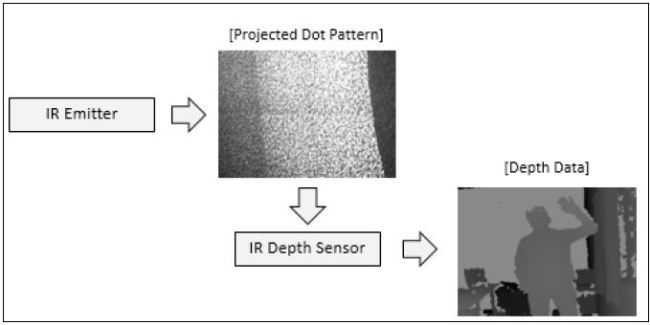
\includegraphics[scale=0.5]{kinect_depth.jpg} }
        \caption{ Kinect depth sensor translating the IR-dot pattern into a 3D representation. }
        \label{fig:kinectIR}
      \end{figure}

    \subsubsection{LIDAR}
      LIDAR (light detection and ranging) sensors uses a laser and its returning time and angle of incidence to determine distance objects relative to the sensor. 
      Most commercial LIDAR devices use a low powered 600-1000 nm laser which is mounted on a motor to pan the laser capturing a single plane.
      A receiver is used to measure the time it takes for the laser to bounce back to the sensor upon encountering an object.
      Their ability to work in varying lighting conditions and ability to detect small objects makes them well suited for use in self-driving cars or autonomous robots. 
      However their limitation to a single plane necessitates other complimentary sensors.

\section{Physical Design}
\label{sec:PhysicalDesign}
  The Logitech Brio webcam provides a high-resolution, two-dimensional image but lacks depth perception.
  The LIDAR provides accurate depth measurement but can only capture point cloud data in a single plane.
  This project proposes bridging the utility of both devices by securing them in stationary positions, then using software to combine their measurements.
  This involves using the M16 LIDAR to get depth sensing information and using computer vision to recognize objects.
  The result is a scalable and reliable depth sensor that will not be affected by natural light, and can be further improved by training a better computer vision model or adding more sensors.
  This project hopes to achieve a proof of concept design to be showcased in a live demo at Oregon State University's 2018 Undergraduate engineering expo.			
  This live demo shall consist of the full system pointed at the project booth's audience. 

  \begin{figure}[h]
    \centering
    \fbox{	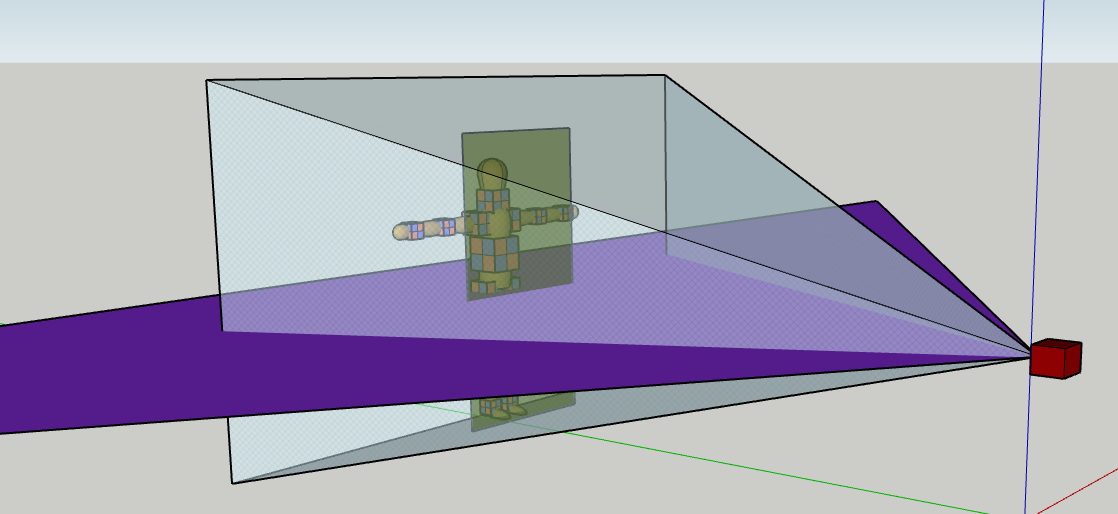
\includegraphics[scale=0.5]{different_dimensions.PNG} }
    \caption{Visualizing different dimensions measured by the LIDAR and Brio Webcam.}
    \label{fig:differentDimensions}
  \end{figure}

  Figure \ref{fig:differentDimensions}  illustrates different dimensions measured by the M16 LIDAR and Brio Webcam.
  The red cube represents the Logitech Brio webcam and M16 LIDAR secured in stationary positions.
  The flat purple triangle represents the M16 LIDAR's horizontal range detection.
  The transparent green rectangle in front of the person represents the computer vision model recognizing that there is a person in-front of the sensor.
  The transparent teal pyramid represents the Brio webcam's field-of-view.

\section{Computer Vision - Dedestrian Detection}
  \subsection{SVM Computer Vision}
  I started with OpenCV's pre-trained facial/pedestrian support-vector-machine (SVM) classifier.
  This SVM is a combination of several other SVMs that detect the upper body, eyes, mouths, and noses.
  The combined SVM is intended to detect faces with high accuracy.
  However, when applied to my design, I could not consistently replicate good results.
  This was due to several factors, namely the SVM used was meant to perform classification on still images where the camera's perspective is far from the subject.

  My design specifications envision a system that quickly tracks multiple subjects in a crowded expo scenario.
  In an expo scenario, human subjects will be moving close or away from the camera, unpredictably shifting their positions, and moving in or out of the field-of-view.
  As seen in \ref{fig:svm}, the OpenCV SVM model does not perform to my specification.
  If the human subject were to turn their head or move too quickly, the SVM will have difficulty tracking their body.
  Additionally, the SVM performs intensive calculations on the computer's CPU, severely limiting the video output's frame-rate and resolution.

  \begin{figure}[h]
    \centering
    \fbox{ 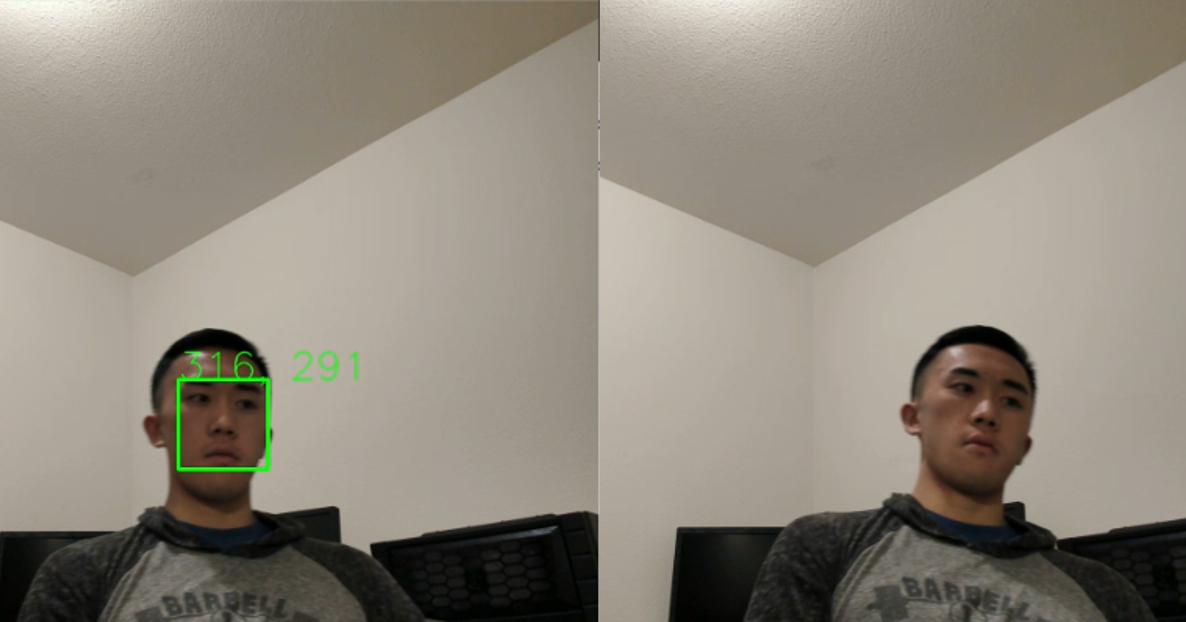
\includegraphics[scale=0.75]{svm.PNG}}
    \caption{figure}{SVM face classification (Left) fails when subject slightly turns their head (Right)}
    \label{fig:svm}
  \end{figure}

  Recognizing the SVM's weaknesses, Tensorflow's open source object detection classifier presented a better computer-vision alternative. \cite{tensorflow}
  The Tensorflow object recognition library is better suited for this project because its library has already been trained to recognize a large dataset of objects. \cite{convolutional_object_detectors}
  These pre-trained datasets in Tensorflow's library are sourced from other machine learning datasets including the COCO dataset, Kitti dataset, and the Open Images dataset. \cite{coco} \cite{open_images} \cite{kitti}

  \begin{figure}[h]
    \centering
    \fbox{  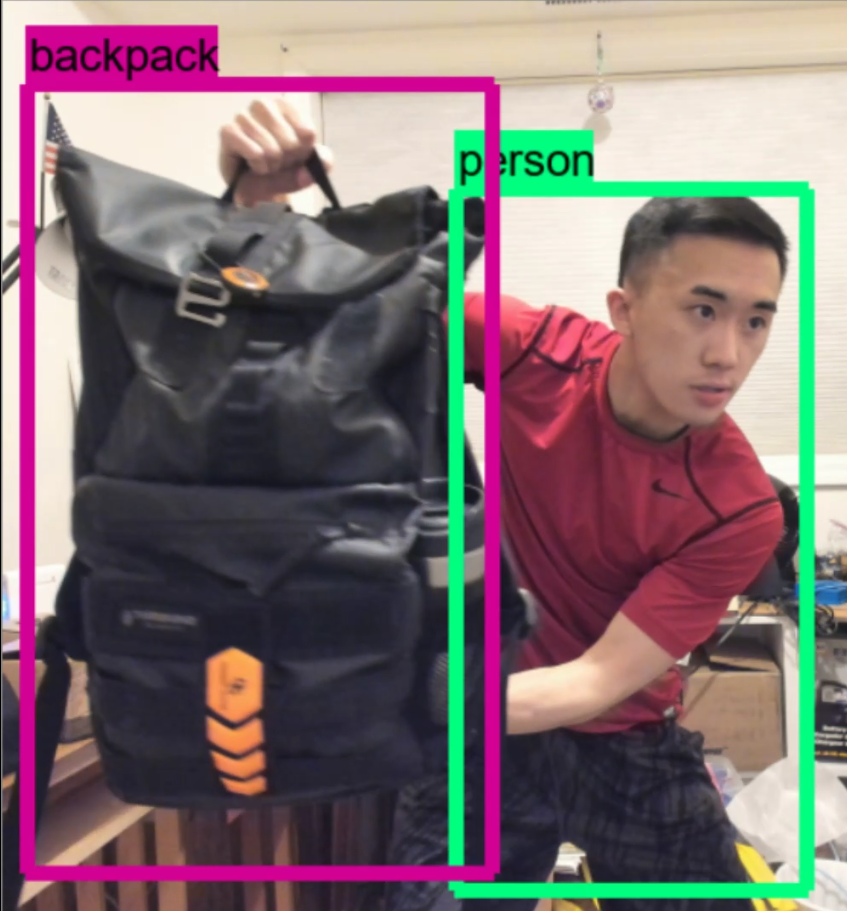
\includegraphics[scale=0.4]{tensorflow.PNG} }
    \caption{figure}{Pre-trained Tensorflow model detecting multiple subjects.}
    \label{tf-detect}
  \end{figure}


  Using this pre-trained Tensorflow model, my project is now able to accurately outline and label over 90 subjects as they come into view of the webcam.
  At the end of Winter Term, the state of the code will enable selectively editing the output video frames to draw bounding boxes on subjects as they move in and out of the camera's field of view.


  Tensorflow also enables us to take advantage of NVIDIA CUDA, a driver that moves intensive calculations to the GPU.
  While this increases the list of material requisitions for demo, moving calculations to the GPU greatly improves the output video quality, frame rate, resolution, and classification speed. \cite{nvidia}



\subsection{Matching Point Cloud Data to Computer Vision Output}

  I developed a work-around to compensate for the slow LIDAR device by splitting the RPLIDAR A1 readings into a seperate thread that pushes data into a shared buffer.
  This allows the Tensorflow model to poll the buffer for new distance data as it needs it.
  However, this work around doesn't completely solve the rotational bottleneck issue. 
  I observed the system's video output dropping to about 25 frames per second.

  Aligning the RPLIDAR A1's laser sweep with the webcam's field of view was a challanging task.
  Upon detecting an object, the RPLIDAR A1 returns several points of incidence consisting of distance and the object's angle with respect to the tip of the device.
  Figure \ref{polar} illustrates the RPLIDAR A1's measurements as a polar plot.
  The tip of the device is considered \( 0^o \), this is an important reference because it splits the usable areas into two hemispheres.
  Through trial and error, I discovered that while in the mount, the RPLIDAR A1's usable area ranged from \( 0^o - 55^o\) and \( 0^o - 305^o\), illustrated as a green triangle in figure \ref{polar}.

  \begin{figure}[h]
    \centering
    \fbox{	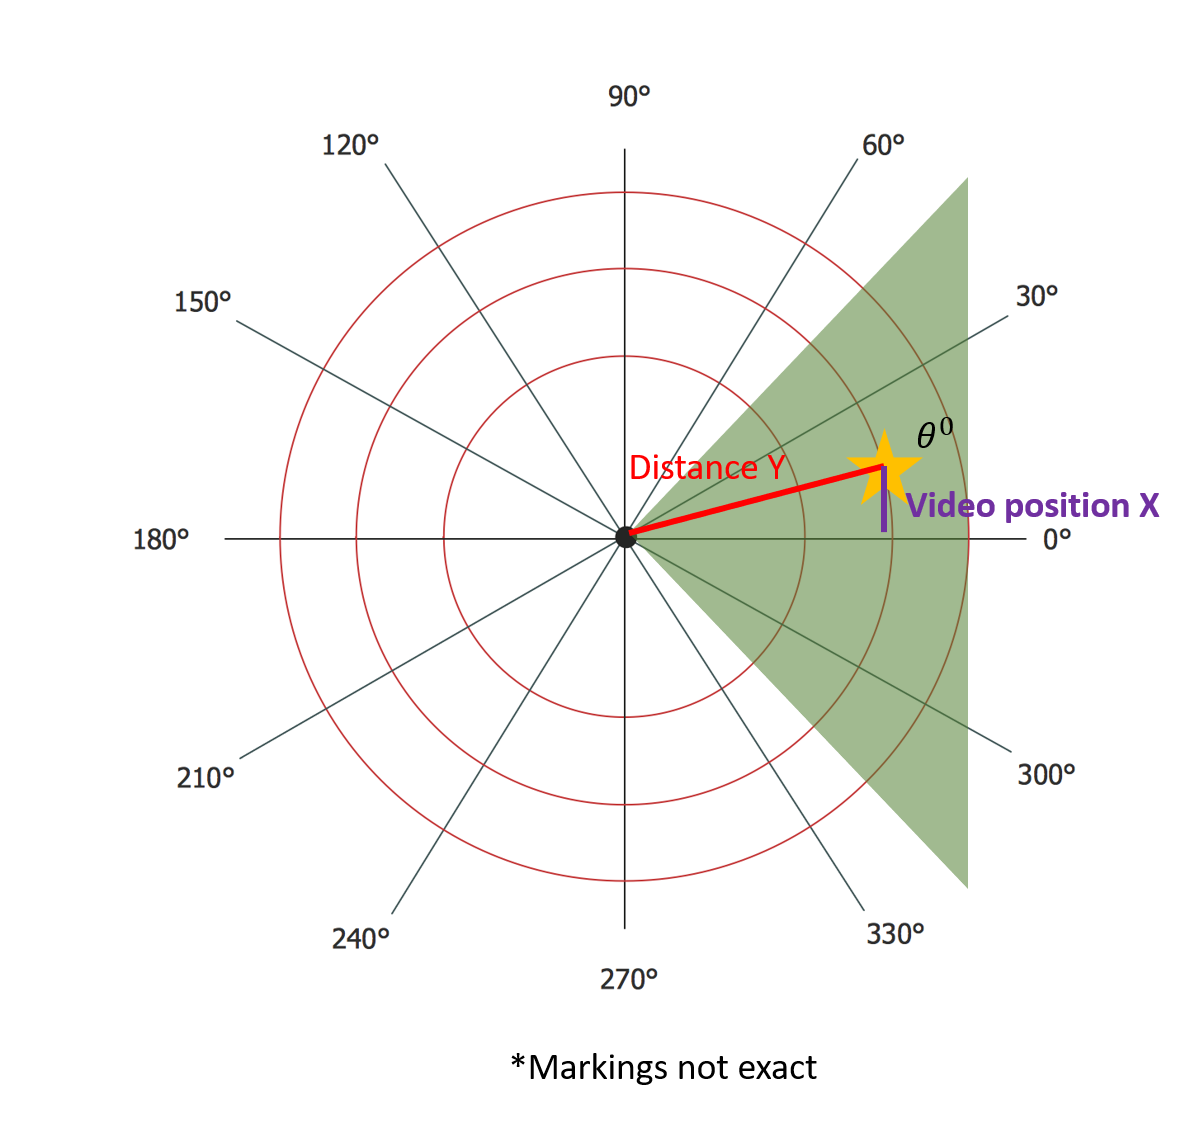
\includegraphics[scale=0.3]{polar.png} }
    \caption{ Polar illustration of the RPLIDAR A1's detection. }
		\label{polar}
  \end{figure}

  One can now use this angle to transpose a point in X-Y dimensions into X-Z video dimensions via similar triangles geometry.
  Let the yellow star in figure \ref{polar} represents a point of incidence that the RPLIDAR A1 detects is at angle \( \theta\).
  One can now use the following equations to translate this point onto the video.

\begin{equation} \label{eq1}
  \theta \leq  55:
  X = \frac{video width}{2} * sin(\theta) + \frac{video width}{2}\\
\end{equation}
\\
\begin{equation} \label{eq2}
  \theta \geq 305:
  X = \frac{video width}{2} * sin(360 - \theta)\\
\end{equation}

Adding an offset \(\frac{video width}{2}\) is necessary because the video output is mirrored as shown in figure \ref{reverse}.


\section{Final System Design}
  The final system consists of the RPLIDAR A1 and Logitech Brio web cam mounted as shown in figure \ref{final_rplidar}.
  During development, it became clear that the RPLIDAR A1 is not an ideal LIDAR device.
  It is a budget hobbyist device whose cost savings significantly affect performance.
  This can be seen in the RPLIDAR's limited range.
  Its sensor/laser assembly fails to reliably detect subjects beyond two meters from the mount. 
  This limits the overall system as subjects must stand within two meters of the system to be properly detected.
  Additionally, the laser experiences significant loss limiting the point aggregation necessary for proper classification.
  As a result, subjects that are broad or are holding large flat objects are more consistently detected.


  I developed a work-around to compensate for the slow LIDAR device by splitting the RPLIDAR A1 readings into a seperate thread that pushes data into a shared buffer.
  This allows the Tensorflow model to poll the buffer for new distance data as it needs it.
  However, this work around doesn't completely solve the rotational bottleneck issue. 
  I observed the system's video output dropping to about 25 frames per second.


  Aligning the RPLIDAR A1's laser sweep with the webcam's field of view was a challanging task.
  Upon detecting an object, the RPLIDAR A1 returns several points of incidence consisting of distance and the object's angle with respect to the tip of the device.
  Figure \ref{polar} illustrates the RPLIDAR A1's measurements as a polar plot.
  The tip of the device is considered \( 0^o \), this is an important reference because it splits the usable areas into two hemispheres.
  Through trial and error, I discovered that while in the mount, the RPLIDAR A1's usable area ranged from \( 0^o - 55^o\) and \( 0^o - 305^o\), illustrated as a green triangle in figure \ref{polar}.

\bibliographystyle{unsrt}  
%\bibliography{references}  %%% Remove comment to use the external .bib file (using bibtex).
%%% and comment out the ``thebibliography'' section.


%%% Comment out this section when you \bibliography{references} is enabled.
\begin{thebibliography}{1}

\bibitem{kour2014real}
George Kour and Raid Saabne.
\newblock Real-time segmentation of on-line handwritten arabic script.
\newblock In {\em Frontiers in Handwriting Recognition (ICFHR), 2014 14th
  International Conference on}, pages 417--422. IEEE, 2014.

\bibitem{kour2014fast}
George Kour and Raid Saabne.
\newblock Fast classification of handwritten on-line arabic characters.
\newblock In {\em Soft Computing and Pattern Recognition (SoCPaR), 2014 6th
  International Conference of}, pages 312--318. IEEE, 2014.

\bibitem{hadash2018estimate}
Guy Hadash, Einat Kermany, Boaz Carmeli, Ofer Lavi, George Kour, and Alon
  Jacovi.
\newblock Estimate and replace: A novel approach to integrating deep neural
  networks with existing applications.
\newblock {\em arXiv preprint arXiv:1804.09028}, 2018.

\end{thebibliography}


\end{document}
